\documentclass{article}
\usepackage{pst-eucl}
\usepackage{changepage, amsmath, amssymb, pgfplots, tikz}
\usetikzlibrary{fit,positioning}
\usepgfplotslibrary{groupplots}
\usepackage[utf8]{inputenc}
\psset{PointName=none,PointSymbol=none}
\usetikzlibrary{arrows.meta}	
\usetikzlibrary{calc,patterns,angles,quotes}
\pgfplotsset{compat=1.16}
\usetikzlibrary{arrows.meta}
\usepackage{fullpage}
\usepackage{xparse,array}
\usepackage{dsfont}
\usetikzlibrary{circuits.ee.IEC}
\usepackage{ulem}
\usepackage{geometry,graphicx}	% Paquetes adicionales.
\usepackage{subcaption,array}
\usepackage{multicol,multirow}
\usepackage{mathtools}
\usepackage{circuitikz,siunitx}
\usepackage{xcolor}
\usetikzlibrary{circuits.ee.IEC}
\usepackage[colorlinks=true, urlcolor=mypurple, linkcolor=mypurple]{hyperref}
\usetikzlibrary{trees}
\usepackage[dvipsnames]{xcolor}
\usepackage{darkmode}
\enabledarkmode
\usepackage{framed} % or, "mdframed"
\usepackage{fancyhdr}
\usepackage{fontawesome}
\pagestyle{fancy}
\usepackage[framed]{ntheorem}
\usepackage{lmodern}
\usepackage{tabularx}
\usepackage{microtype}
\setlength{\columnsep}{1.5cm}
\setlength{\columnseprule}{0.4pt}
\usepackage{multicol}
\usetikzlibrary{arrows, shapes.gates.logic.US, calc}
\usetikzlibrary{calc,arrows.meta}
\usepackage{tcolorbox}
\usepackage{pst-node}% http://ctan.org/pkg/pst-node
\definecolor{p1}{HTML}{caf0f8}
\definecolor{p2}{HTML}{ade8f4}
\definecolor{p3}{HTML}{90e0ef}
\definecolor{p4}{HTML}{48cae4}
\definecolor{p5}{HTML}{00b4d8}
\definecolor{p6}{HTML}{0096c7}
\definecolor{p7}{HTML}{0077b6}
\definecolor{p8}{HTML}{023e8a}
\definecolor{p9}{HTML}{03045e}
\usepackage{multicol}
\usepackage{colortbl}
\colorlet{xcol}{blue!60!black}
\usepackage{capt-of}
\definecolor{myred}{HTML}{f44336}
\definecolor{mypink}{HTML}{e81e63}
\definecolor{mypurple}{HTML}{9c27b0}
\definecolor{mydeeppurple}{HTML}{673ab7}
\definecolor{myindigo}{HTML}{3f51b5}
\definecolor{myblue}{HTML}{2196f3}
\definecolor{mylightblue}{HTML}{03a9f4}
\definecolor{mycyan}{HTML}{00bcd4}
\definecolor{myteal}{HTML}{009688}
\definecolor{mygreen}{HTML}{4caf50}
\definecolor{mylightgreen}{HTML}{8bc34a}
\definecolor{mylime}{HTML}{cddc39}
\definecolor{myyellow}{HTML}{ffeb3b}
\definecolor{myamber}{HTML}{ffc107}
\definecolor{myorange}{HTML}{ff9800}
\definecolor{mydeeporange}{HTML}{ff5722}
\definecolor{mybrown}{HTML}{795548}
\definecolor{mygray}{HTML}{9e9e9e}
\definecolor{mybluegray}{HTML}{607d8b}
\definecolor{pag}{HTML}{293133}
\usepackage[labelformat=empty]{caption}
\usepackage{mdframed}
\newtcolorbox{qq}[2][]{%
	boxrule=0.75pt,
	sharp corners,  % Square edges
	colframe=white,  % Set the color of the outline
	colback=pag,  % Set the color of the fill
	coltext=white,
	#1,
}
\newframedtheorem{frm-thm}{Theorem}

\usepackage{tikz-3dplot}
\usetikzlibrary{3d,backgrounds,intersections}
% small fix for canvas is xy plane at z % https://tex.stackexchange.com/a/48776/121799
\makeatletter
\tikzoption{canvas is xy plane at z}[]{%
	\def\tikz@plane@origin{\pgfpointxyz{0}{0}{#1}}%
	\def\tikz@plane@x{\pgfpointxyz{1}{0}{#1}}%
	\def\tikz@plane@y{\pgfpointxyz{0}{1}{#1}}%
	\tikz@canvas@is@plane}
\makeatother

\usepgfplotslibrary{groupplots}

\tikzset{
	conditional line/.style 2 args={
		/utils/exec={\pgfmathsetmacro{\xcoordA}{#1}},
		/utils/exec={\pgfmathsetmacro{\xcoordB}{#2}},
		insert path={
			\ifdim\xcoordA pt>\xcoordB pt
			(\xcoordA,0) -- (\xcoordB,0)
			\fi
		},
	},
}

\newcommand{\Logo}{
	\begin{tikzpicture}[remember picture,overlay]
		\node at ($(current page.north east) + (-1cm,-1cm)$) {AC};
	\end{tikzpicture}
}




%--------------------------------------------------------------------



\newcommand{\framedtext}[1]{%
	\par%
	\noindent\fbox{%
		\parbox{\dimexpr\linewidth-2\fboxsep-2\fboxrule}{#1}%
	}%
}


\tikzset{
	venn box/.style={
		draw=black, very thick, 
		rounded corners=10,
		inner xsep=10pt, inner ysep=15pt, outer ysep=5pt
	},
	venn numbers/.style={
		%    draw,
		inner ysep=0pt,
		align=center
	},
	venn title/.style={
		fill=black, text=white
	}
}


\ExplSyntaxOn
\NewDocumentCommand{\truthtable}{mm}
{
	\group_begin:
	\setlength{\arraycolsep}{0pt}
	\crocket_truth_make_preamble:n { #1 }
	\crocket_truth_make_body:n { #2 }
	\crocket_truth_make:
	\group_end:
}

% variables
\tl_new:N \l__crocket_truth_preamble_tl
\tl_new:N \l__crocket_truth_first_tl
\tl_new:N \l__crocket_truth_body_tl
\seq_new:N \l__crocket_truth_rows_seq

% internal functions
\cs_new_protected:Nn \crocket_truth_make_preamble:n
{
	\tl_clear:N \l__crocket_truth_preamble_tl
	\tl_clear:N \l__crocket_truth_first_tl
	% examine the first argument in order to build the table
	% preamble and the first row
	\tl_map_inline:nn { #1 }
	{
		\tl_if_in:VnTF \c_crocket_truth_delims_tl { ##1 }
		{% a delimiter is inserted in @{...} as a phantom (almost)
			% and not taken into account for the first row
			\tl_put_right:Nn \l__crocket_truth_preamble_tl { @{ \__crocket_truth_delim:n {##1} } }
		}
		{
			\tl_if_eq:nnTF { | } { ##1 }
			{% vertical bar is ignored in the rows, but it gives a | in
				% the table preamble (actually, quad | quad)
				\tl_put_right:Nn \l__crocket_truth_preamble_tl { @{\hspace{1em}}|@{\hspace{1em}} }
			}
			{% otherwise, c is added to the table preamble and
				% the item to the first row
				\tl_put_right:Nn \l__crocket_truth_preamble_tl { c }
				\tl_put_right:Nn \l__crocket_truth_first_tl { ##1 & }
			}
		}
	}
	% since rows will end with &, we add a dummy trailing column
	\tl_put_right:Nn \l__crocket_truth_preamble_tl { c } % empty last column
}

\cs_new_protected:Nn \crocket_truth_make_body:n
{% start building the table body
	\tl_clear:N \l__crocket_truth_body_tl
	% split the argument at \\
	\seq_set_split:Nnn \l__crocket_truth_rows_seq { \\ } { #1 }
	% and map it
	\seq_map_inline:Nn \l__crocket_truth_rows_seq
	{% each item is a row; map it to add &
		\tl_map_inline:nn { ##1 }
		{% but ignoring |
			\tl_if_eq:nnF { | } { ####1 }
			{
				\tl_put_right:Nn \l__crocket_truth_body_tl { \crocket_truth_tf:n { ####1 } & }
			}
		}
		% append the row terminator
		\tl_put_right:Nn \l__crocket_truth_body_tl { \\ }
	}
}

\cs_new_protected:Nn \crocket_truth_make:
{% make the table
	\exp_args:NnV \begin {array} \l__crocket_truth_preamble_tl
	% temporary define \__crocket_truth_delim:n to produce its argument
	\noalign { \cs_gset_eq:NN \__crocket_truth_delim:n \use:n }
	% output the first row
	\tl_use:N \l__crocket_truth_first_tl \\
	\hline
	% make \__crocket_truth_delim:n to deliver a phantom
	\noalign { \cs_gset_eq:NN \__crocket_truth_delim:n \hphantom }
	\tl_use:N \l__crocket_truth_body_tl
\end{array}
}

\cs_new_protected:Nn \crocket_truth_tf:n { \makebox[1.2em]{ $ \mathrm { #1 }$ } }

\tl_const:Nn \c_crocket_truth_delims_tl { ()[]\{\} }

\ExplSyntaxOff


%--------------------------------------------------------------------
\newcommand{\bs}{\textcolor{bluefill}{'}}
\definecolor{bluefill}{RGB}{41, 49, 51}
\renewcommand\columnseprulecolor{\hspace{50pt}}

% PROPIEDAD DISTRIGUTIVA COMANDO DE FLECHAS
\newcommand\source[1]{%
	\tikz[remember picture,baseline,inner sep=0pt] {%
		\node [name=source,anchor=base]{$#1$};
	}%
	\setcounter{target}{0}
}

\newcounter{target}
\newcommand\target[1]{%
	\tikz[remember picture,baseline,inner sep=0pt] {%
		\node [name=target-\thetarget,anchor=base]{$#1$};
	}%
	\stepcounter{target}%
}

\newcommand\drawarrows{
	\tikz[remember picture, overlay, bend left=20, -latex] {
		\foreach \i [evaluate=\i as \n using int(\i-1)] in {1,...,\thetarget} {
			\draw (source.north) to (target-\n.north);
		}
	}
}

% Portrail


\title{Algebra I}
\date{\today}
\author{Alejandro Ceccheto}



\begin{document}
	%% School Portrail.
	\maketitle
	\pagebreak
	
	

	\begin{frm-thm}[Proposiciones Lógicas]
		Si un número es par entonces es múltiplo de 3 \\
		\begin{center}
			x par $\Rightarrow$ x mult. de 3
		\end{center}
	\end{frm-thm}


	
	
	
\begin{multicols}{3}
	\begin{minipage}[t]{0.5\textwidth}
		\fbox{p, q, r} = Proposiciones. \\
		
		\begin{itemize}
			\item 1, 0 $\rightarrow$ prop. \\
			
			\item 1 y 0 $\rightarrow$ p $\land$ q\\
			
			\item 1 o 0 $\rightarrow$ p $\lor$ q \\
			
			\item o 1 o 0 $\rightarrow$ p $\veebar$ q \\
			
			\item si 1 entonces 0 $\rightarrow$ p $\Longrightarrow$ q \\
			
			\item equivalencia $\rightarrow$ p $\Longleftrightarrow$ q \\
			
			\item Negación $\rightarrow$  $>$p, $\vec{p}$, $\sim$p, -p \\
		\end{itemize}
	\end{minipage}
	
	Negación =
	\begin{minipage}{0.5cm}
		\[
		\truthtable{
			P | \sim P
		}{
			V | F \\
			F | V
		}
		\]
	\end{minipage}
	
	Conjunción =
	\begin{minipage}[c]{0.5cm}
		\[
		\truthtable{
			P Q | P \land Q
		}{  V V | \bs V \\
		    V F | \bs F \\
		    F V | \bs F \\
		    F F | \bs F \\
		}
		\]
	\end{minipage}
	
	
    Disyunción = 
	\begin{minipage}[c]{0.5cm}
		\[
		\truthtable{
			P Q | P \lor Q
		}{  V V | \bs V \\
		    F V | \bs V \\
		    V F | \bs V \\
		    F F | \bs F \\
		}
		\]
		
	\end{minipage}
	                                                                                          
	
	Condicional =
	\begin{minipage}[c]{1cm}
		\[
		\truthtable{ P Q | P \Rightarrow Q
		}{           V V | \bs V \\
		             V F | \bs F \\
		             F V | \bs V \\
		             F F | \bs V \\
		}
		\]
	\end{minipage}
	
	
	Bicondicional= 
	\begin{minipage}[c]{1cm}
		\[
		\truthtable{P Q	| P \Leftrightarrow Q 
		}{ V V | \bs V \\
		   V F | \bs F \\
		   F V | \bs F \\
		   F F | \bs V \\
		}
		\]
	\end{minipage}
\end{multicols}

Entonces, con estas lógicas algebraicas podemos deducir 3 cosas, si son Tautología, que significa que siempre va a ser verdadero, Contradicción, que significa que son siempre falsas, o Contingencia $\rightarrow$ a veces V, otras F.

\begin{multicols}{2}
	\begin{minipage}{0.5\textwidth}
		\[
		\truthtable{
			P Q | r | P \lor Q | P \lor Q \Rightarrow r  
		}{  V V V \bs V \bs \bs V \bs \bs \\
			V V F \bs V \bs \bs F \bs \bs \\
			V F V \bs F \bs \bs V \bs \bs \\
			V F F \bs F \bs \bs V \bs \bs \\
			F V V \bs F \bs \bs V \bs \bs \\
			F V F \bs F \bs \bs V \bs \bs \\
			F F V \bs F \bs \bs V \bs \bs \\
			F F F \bs F \bs \bs V
		}
		\]
	\end{minipage}
	
	\begin{tikzpicture}
	\node {$\sim$p$\lor$q}
	[edge from parent fork left,grow=left]
	child {node {q}}
	child {node {$\sim$p}
		child {node {p}}
	};
	\node [below right, text width=10cm,align=justify] at (1,-0.5)
	{ (por cultura general)
	};
\end{tikzpicture}
\end{multicols}
\pagebreak

\vspace{-1.2cm}
\section{Ejericios hechos.}

\vspace{0.5cm}


\begin{itemize}
	\item[1. ] $\sim$(p$\lor$q)

\[
\truthtable{
	P Q | P \lor Q | \sim (p\lor q)
}{  
	V V | \bs V \bs\bs F \\
	F V | \bs V \bs\bs F \\
	V F | \bs V \bs\bs F \\
	F F | \bs F \bs\bs V 
}
\]



\item[2. ]P$\Rightarrow$(q$\land$$\sim$q)
\[
\truthtable{
	P Q | \sim Q | (Q \land \sim P) | P \Rightarrow (Q \land \sim Q)
}{  
	V V | \bs F \bs F \bs\bs\bs\bs F \\
	V F | \bs V \bs F \bs\bs\bs\bs F \\
	F V | \bs F \bs F \bs\bs\bs\bs V \\
	F F | \bs V \bs F \bs\bs\bs\bs V
}
\]

\item[3. ] p $\Rightarrow$ (q $\lor$ $\sim$ q)
\[
\truthtable{
	P Q | \sim Q | (Q \lor \sim Q) | P \Rightarrow (Q \lor \sim Q)
}{  V V | \bs F \bs  V \bs  \bs  \bs \bs V \\
    V F | \bs V \bs  V \bs  \bs  \bs \bs V \\
    F V | \bs F \bs  V \bs  \bs  \bs \bs V \\
    F F | \bs V \bs  V \bs  \bs  \bs \bs V \\
} 
\]
\end{itemize}


Para mas referencias y ejemplos visitar\footnote{Uno de los libros que mas se asemeja a la forma de explicar de la profe. \\
\url{https://archive.org/details/AlgebraIArmandoRojo/page/n13/mode/2up}}.



 \section*{Chapter 2: Propiedades.}

En este capitulo veremos como se aplican las propiedades en álgebra, particularmente en proposiciones.
Para eso particularmente a mi tendriamos que tener en mente las 3 tablas de y,ó e implica.

\begin{center}
	\[
	\truthtable{
		P Q | P \land Q
	}{  V V | \bs V \bs \\
	}
	\]
	\[
	\truthtable{
		P Q | P \lor Q
	}{  F F | \bs F \bs \\
	}
	\]
	\[
	\truthtable{
		P Q | P \Rightarrow Q
	}{  V F | \bs F \bs \\
	}
	\]
\end{center}


\section{Propiedades.}
Estas son las 3 cosas que tendríamos que tener en mente siempre al momento de operar con condicionales.
Luego las propiedades hay bastantes una leve lista de ellas seria.

\begin{itemize}
	\item Propiedad conmutativa.
	\item Propiedad Distributiva.
	\item Propiedad Absorción.
	\item Propiedad Semis-Absorción.
	\item Propiedad de Morgan.
\end{itemize}
Entre muchas otras, estas son las que mas se suelen usar.

\subsection*{Propiedad Distributiva.}

\begin{frm-thm}
	\begin{equation*}
		P \land(Q \lor R) \equiv (P \land Q) \lor (P \lor Q)
	\end{equation*}
	lo que platea la teoria es que $P$ y (Q O R) es equivalente a (P y R) ó (P ó Q) siendo que la $P$ se reparte entre Q y R.
\end{frm-thm}


\vspace{1cm}
	\subsubsection*{Ejemplo}
\begin{center}
	$\source{(P\lor(Q\vee R))} \equiv \big( \target{(P \land Q)} \lor \target{(P \vee R)} \big)$\drawarrows
\end{center}

\subsection*{Propiedad Asociativa.}

\begin{frm-thm}
	\begin{gather*}
		\big((P \vee Q) \vee R  \big) \equiv \big(P \vee (Q \vee R)\big) \\
		\big((P \land Q) \land R\big) \equiv \big(p \land (Q \land R)\big)
	\end{gather*}
     Planteo de la propiedad, es lo mismo escribir ($P$ ó $Q$) ó $R$ $\Leftrightarrow$ $P$ ó ($Q$ ó $R$) lo mismo sucede si tenemos y´s ($\land$).
\end{frm-thm}

\section{Propiedades.}

\begin{frm-thm}
	\begin{gather*}
		\big(P \land Q\big) \equiv \big(Q \land P\big) \\
		\big(P \vee Q\big) \equiv \big(Q \vee P\big) \\
		\big(P \Leftrightarrow Q \big) \equiv \big(Q \Leftrightarrow P\big) \\
		\big(P \veebar Q\big) \equiv \big(Q \veebar P\big)
	\end{gather*}
	 La propiedad plantea que siempre se puede escribir de distinta forma una operacion simepre y cuando esta sea llevada a la simpleza de $n$ y/o/im/ $n$.
\end{frm-thm}

\vspace{0.5cm}

\subsection*{Negación de \textbf{$\underbrace{Conujuncion / Diyuncion}_\textrm{Propiedad de Morgan}$}.}

\vspace{0.5cm}

 \begin{frm-thm}
 	Esta propiedad plantea que si tengo una negación antes que un conjunto, dicha negacion puede negar los dos conjuntos por separado e invertir su unión ($\vee, \land, \Leftarrow$)
 	\begin{gather*}
 		\sim\big(P \vee Q\big) \equiv \sim P \land \sim Q \\
 		\sim\big(P \land Q\big) \equiv \sim P \vee \sim Q
 	\end{gather*}
 \end{frm-thm}

\subsection*{Absorción y Semi-Absorción.}

\begin{center}
	\begin{tabular}{ | l | l  | p{5cm} |}
		\hline
		F = Contradiccion & V = Tautologia \\ \hline
		$\sim\big(\sim P\big) \equiv P$ & $P \vee \mathds{V} \equiv \mathds{V}$                                           \\ \hline
		 --- & $P \hspace{3pt}\vee \sim P \equiv \mathds{V}$  \\ \hline
		$P \hspace{3pt}\land \sim P \equiv \mathds{F}$ &---   \\ \hline
		$P \hspace{3pt}\land \mathds{F} \equiv F$ &  ---      \\ \hline
		$P \hspace{3pt}\lor \mathds{F} \equiv P$ & ---        \\
		
		\hline
	\end{tabular}
\end{center}

\pagebreak
\section{Propiedades.}

\vspace{0.9cm}

\subsection*{Propiedades de absorción.}
%% This block is what you'll need to put in your code where you want your picture.
\begin{center}
	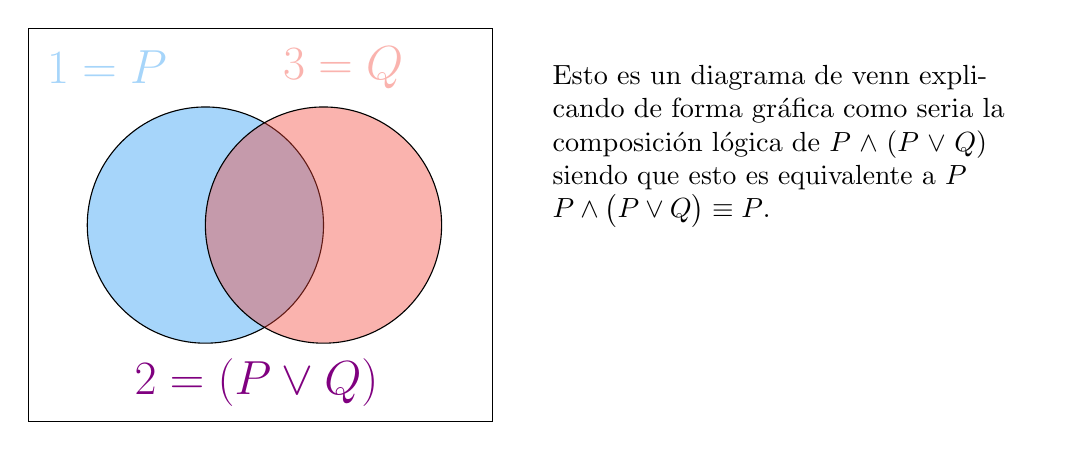
\begin{tikzpicture}[scale=0.5pt]
		%% You can adjust the opacity here. For venn diagrams it is convenient to have a low opacity so that you can see intersections
		\begin{scope} [fill opacity = .4]
			%% The draw command knows a lot of shapes. To make a rectangle you just need to specify two diagonal corners. Make sure you always have a semicolon at the end of your draw commands, otherwise latex flips out.
			\draw (-5,6) rectangle (6.8,-4);
			%% Similarly, you can make a circle by specifying the center and then the radius. You can also add a fill color, but if you're printing in black and white you'll probably want to remove that line.
			\draw[fill=myblue, draw = black] (-0.5,1) circle (3);
			\draw[fill=myred, draw = black] (2.5,1) circle (3);
			%% We can use the node command to label points. If you put your cursor on "LARGE" or "textbf" a box will drop down with size and text style options.
			\node[color=myblue] at (-3,5) {\LARGE\textbf{$1 = P $}};
			\node[color=myred] at (3,5) {\LARGE\textbf{$3 = Q$}};
		\end{scope}
		\node[color=violet] at (0.8,-3){\LARGE\textbf{$2 =(P \vee Q)$}};
		\node at (6,3) [right=1cm,text width=6cm,rounded corners,inner sep=1ex,]
		{Esto es un diagrama de venn explicando de forma gráfica como seria la composición lógica de $P \land (P \vee Q)$ siendo que esto es equivalente a $P$ \\
			$P \land \big(P \vee Q\big) \equiv P$.};
		%% And now you have a venn diagram. Yay!
		%\draw[help lines](-5,5) grid (5,-6);    This line can draw the grid lines to help guide you. I use these when I'm writing the code and then delete this line when I publish the pdf.
	\end{tikzpicture}
	
	\vspace{6pt}
	%% This block is what you'll need to put in your code where you want your picture.
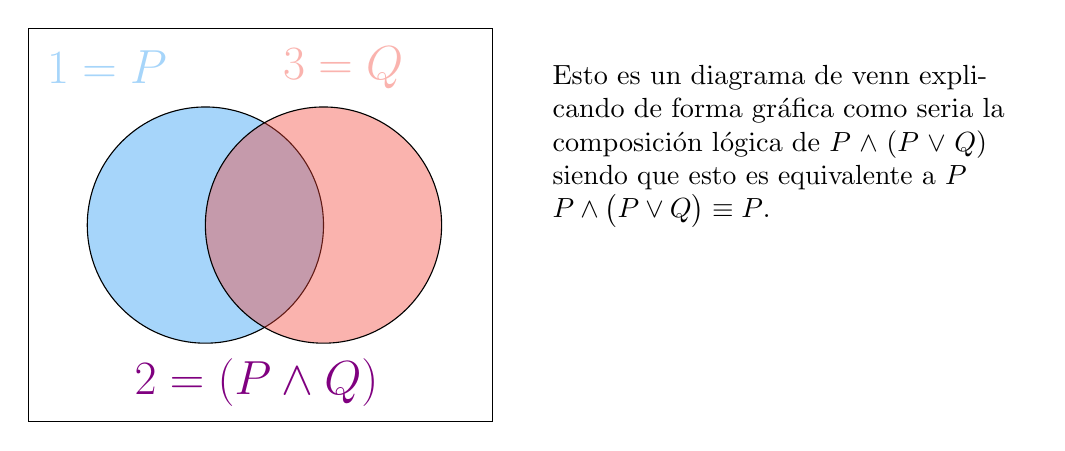
\begin{tikzpicture}[scale=0.5pt]
	%% You can adjust the opacity here. For venn diagrams it is convenient to have a low opacity so that you can see intersections
	\begin{scope} [fill opacity = .4]
		%% The draw command knows a lot of shapes. To make a rectangle you just need to specify two diagonal corners. Make sure you always have a semicolon at the end of your draw commands, otherwise latex flips out.
		\draw (-5,6) rectangle (6.8,-4);
		%% Similarly, you can make a circle by specifying the center and then the radius. You can also add a fill color, but if you're printing in black and white you'll probably want to remove that line.
		\draw[fill=myblue, draw = black] (-0.5,1) circle (3);
		\draw[fill=myred, draw = black] (2.5,1) circle (3);
		%% We can use the node command to label points. If you put your cursor on "LARGE" or "textbf" a box will drop down with size and text style options.
		\node[color=myblue] at (-3,5) {\LARGE\textbf{$1 = P $}};
		\node[color=myred] at (3,5) {\LARGE\textbf{$3 = Q$}};
	\end{scope}
	\node[color=violet] at (0.8,-3){\LARGE\textbf{$2 =(P \land Q)$}};
	
	\node at (6,3) [right=1cm,text width=6cm,rounded corners,inner sep=1ex,]
	{Esto es un diagrama de venn explicando de forma gráfica como seria la composición lógica de $P \land (P \vee Q)$ siendo que esto es equivalente a $P$ \\
		$P \land \big(P \vee Q\big) \equiv P$.};
	%% And now you have a venn diagram. Yay!
	%\draw[help lines](-5,5) grid (5,-6);    This line can draw the grid lines to help guide you. I use these when I'm writing the code and then delete this line when I publish the pdf.
\end{tikzpicture}
\end{center}

\pagebreak

\subsection*{Propiedades de Semi-Absorción.}


\begin{center}
	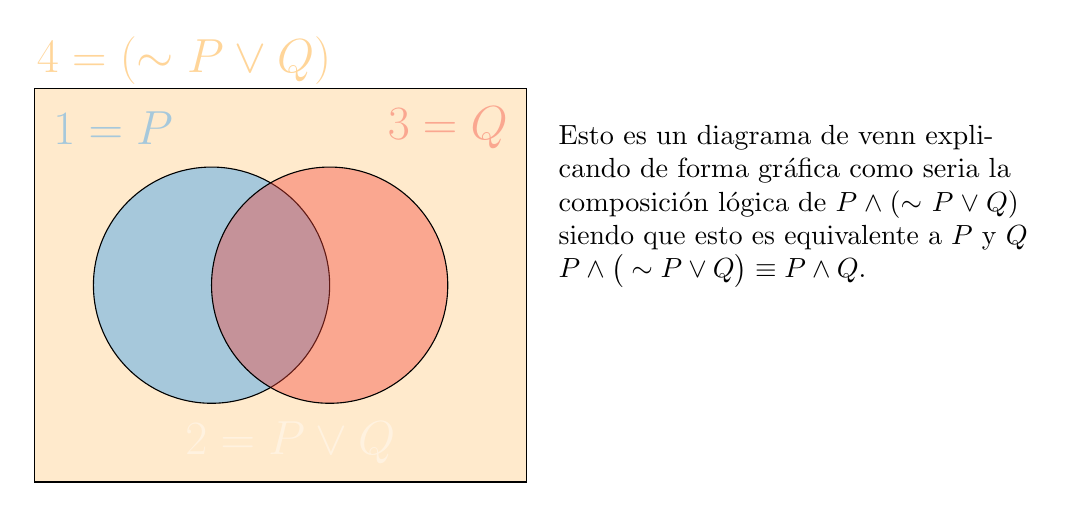
\begin{tikzpicture}[scale=0.5pt]
		%% You can adjust the opacity here. For venn diagrams it is convenient to have a low opacity so that you can see intersections
		\begin{scope} [fill opacity = .4]
			%% The draw command knows a lot of shapes. To make a rectangle you just need to specify two diagonal corners. Make sure you always have a semicolon at the end of your draw commands, otherwise latex flips out.
			\draw[fill opacity=.2, fill=myorange] (-5,6) rectangle (7.5,-4);
			%% Similarly, you can make a circle by specifying the center and then the radius. You can also add a fill color, but if you're printing in black and white you'll probably want to remove that line.
			\draw[fill=myblue, draw = black] (-0.5,1) circle (3);
			\draw[fill=myred, draw = black] (2.5,1) circle (3);
			%% We can use the node command to label points. If you put your cursor on "LARGE" or "textbf" a box will drop down with size and text style options.
			\node[color=myblue] at (-3,5) {\LARGE\textbf{$1 = P$}};
			\node[color=white] at (1.5,-3) {\LARGE\textbf{$2 = P \vee Q$}};
			\node[color=myorange] at (-1.2,6.7) {\LARGE\textbf{$4 = (\sim P\lor Q)$}};
			\node[color=myred] at (5.5,5) {\LARGE\textbf{$3 = Q$}};
		\end{scope}
		\node at (6,3) [right=1cm,text width=6cm,rounded corners,inner sep=1ex,]
		{Esto es un diagrama de venn explicando de forma gráfica como seria la composición lógica de $P \land (\sim P \vee Q)$ siendo que esto es equivalente a $P$ y $Q$ \\
			$P \land \big(\sim P \vee Q\big) \equiv P\land Q$.};
		%% And now you have a venn diagram. Yay!
		%\draw[help lines](-5,5) grid (5,-6);    This line can draw the grid lines to help guide you. I use these when I'm writing the code and then delete this line when I publish the pdf.
	\end{tikzpicture}
	
	\vspace{6pt}
	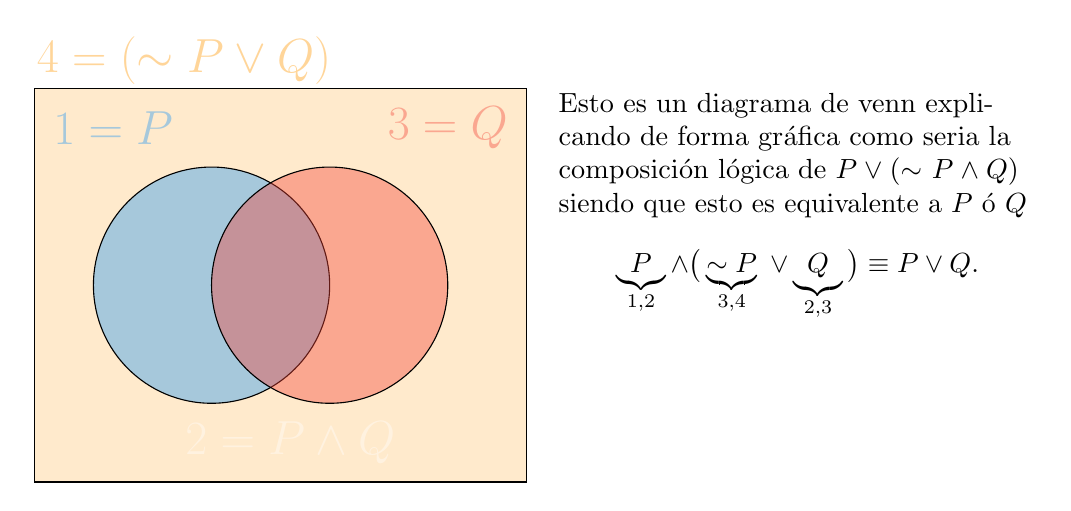
\begin{tikzpicture}[scale=0.5pt]
		%% You can adjust the opacity here. For venn diagrams it is convenient to have a low opacity so that you can see intersections
		\begin{scope} [fill opacity = .4]
			%% The draw command knows a lot of shapes. To make a rectangle you just need to specify two diagonal corners. Make sure you always have a semicolon at the end of your draw commands, otherwise latex flips out.
			\draw[fill opacity=.2, fill=myorange] (-5,6) rectangle (7.5,-4);
			%% Similarly, you can make a circle by specifying the center and then the radius. You can also add a fill color, but if you're printing in black and white you'll probably want to remove that line.
			\draw[fill=myblue, draw = black] (-0.5,1) circle (3);
			\draw[fill=myred, draw = black] (2.5,1) circle (3);
			%% We can use the node command to label points. If you put your cursor on "LARGE" or "textbf" a box will drop down with size and text style options.
			\node[color=myblue] at (-3,5) {\LARGE\textbf{$1 = P$}};
			\node[color=white] at (1.5,-3) {\LARGE\textbf{$2 = P \land Q$}};
			\node[color=myorange] at (-1.2,6.7) {\LARGE\textbf{$4 = (\sim P\lor Q)$}};
			\node[color=myred] at (5.5,5) {\LARGE\textbf{$3 = Q$}};
		\end{scope}
		\node at (6,3) [right=1cm,text width=6cm,rounded corners,inner sep=1ex,]
		{Esto es un diagrama de venn explicando de forma gráfica como seria la composición lógica de $P \vee (\sim P \land Q)$ siendo que esto es equivalente a $P$ ó $Q$ \\
		\begin{center}
				$\underbrace{P}_\textrm{1,2} \land \big(\underbrace{\sim P}_\textrm{3,4} \hspace{3pt} \vee \underbrace{Q}_\textrm{2,3}\big) \equiv P\vee Q$.
		\end{center}
		};
		%% And now you have a venn diagram. Yay!
		%\draw[help lines](-5,5) grid (5,-6);    This line can draw the grid lines to help guide you. I use these when I'm writing the code and then delete this line when I publish the pdf.
	\end{tikzpicture}
\end{center}

\subsection*{Propiedad de morgan.}


\begin{frm-thm}
	Esta propiedad se mete con los implica $\Rightarrow$, de forma que podemos convertirlos en expresiones mucho mas faciles de resolver sin tener que pensar en la tabla del implica.
	\begin{center}
		\begin{equation*}
			\big(P \Rightarrow Q\big) \equiv \big(\sim P \vee Q\big)
		\end{equation*}
	\end{center}
\end{frm-thm}

\pagebreak

\section*{Ejercicio hecho.}
\subsubsection*{Ejercicio de ejemplo.}

\begin{gather*}
	\sim\big(Q \Rightarrow P\big) \Rightarrow \big((P \vee Q) \Rightarrow (Q \land \sim P)\big) 
\end{gather*}

\begin{gather*}
	\underbrace{\sim\big(Q \Rightarrow P\big)}_\textrm{P} \Rightarrow \underbrace{\big((P \vee Q) \Rightarrow (Q \land \sim P)\big)}_\textrm{Q}
\end{gather*}

\begin{gather}
	\sim\big(Q \Rightarrow P\big) \Rightarrow \big((P \vee Q) \Rightarrow (Q \land \sim P)\big) \\
	\sim(Q \vee P) \vee \big((P \vee Q) \Rightarrow (Q \land \sim P)\big) \\
	\sim(Q \vee P) \vee \big(\sim(P \vee Q) \vee (Q \land \sim P) \big) \\
	\sim(\sim Q \vee \sim P) \vee \big((\sim P \land \sim Q) \vee (Q \land \sim P)\big) \\
	(Q \land \sim P) \vee \big((\sim P \land \sim Q) \vee (\sim P \land Q)\big) \\
	\sim P \land (\sim Q \vee Q) \\
	\sim P \land \mathds{V} \equiv Absorcion \\
	(\sim P \land Q) \vee \sim P \equiv \sim P
\end{gather} En\footnote[2]{Fecha de modificación y adición al 2/4/2024}











\end{document}